%!TEX root = prelim.tex
%!TEX root = fakeroot.tex

\frame{
\frametitle{Combining MRF recognition with alignment}
\begin{itemize}
\item Already demonstrated improved performance with SRC + Alignment and also with SRC + MRF.
\item Need to demonstrate that SRC + Alignment + MRF can work
\item Implementation: Iterate between solving:

\begin{enumerate}
\item $\min_{\x,\e,\Delta\tau_i \in T} \| \e \|_1 \quad \subj \quad \y\circ \tau + J \Delta \tau_i = A_i \x + \e \textrm{ on } \s$
\item $\max_{\s}  \sum_{(i,j)\in E}  \lambda \s[i]\s[j] + \sum_{i\in V} \log p(\e[i] | \s[i]).$
\end{enumerate}
\end{itemize}

\begin{center}
\fbox{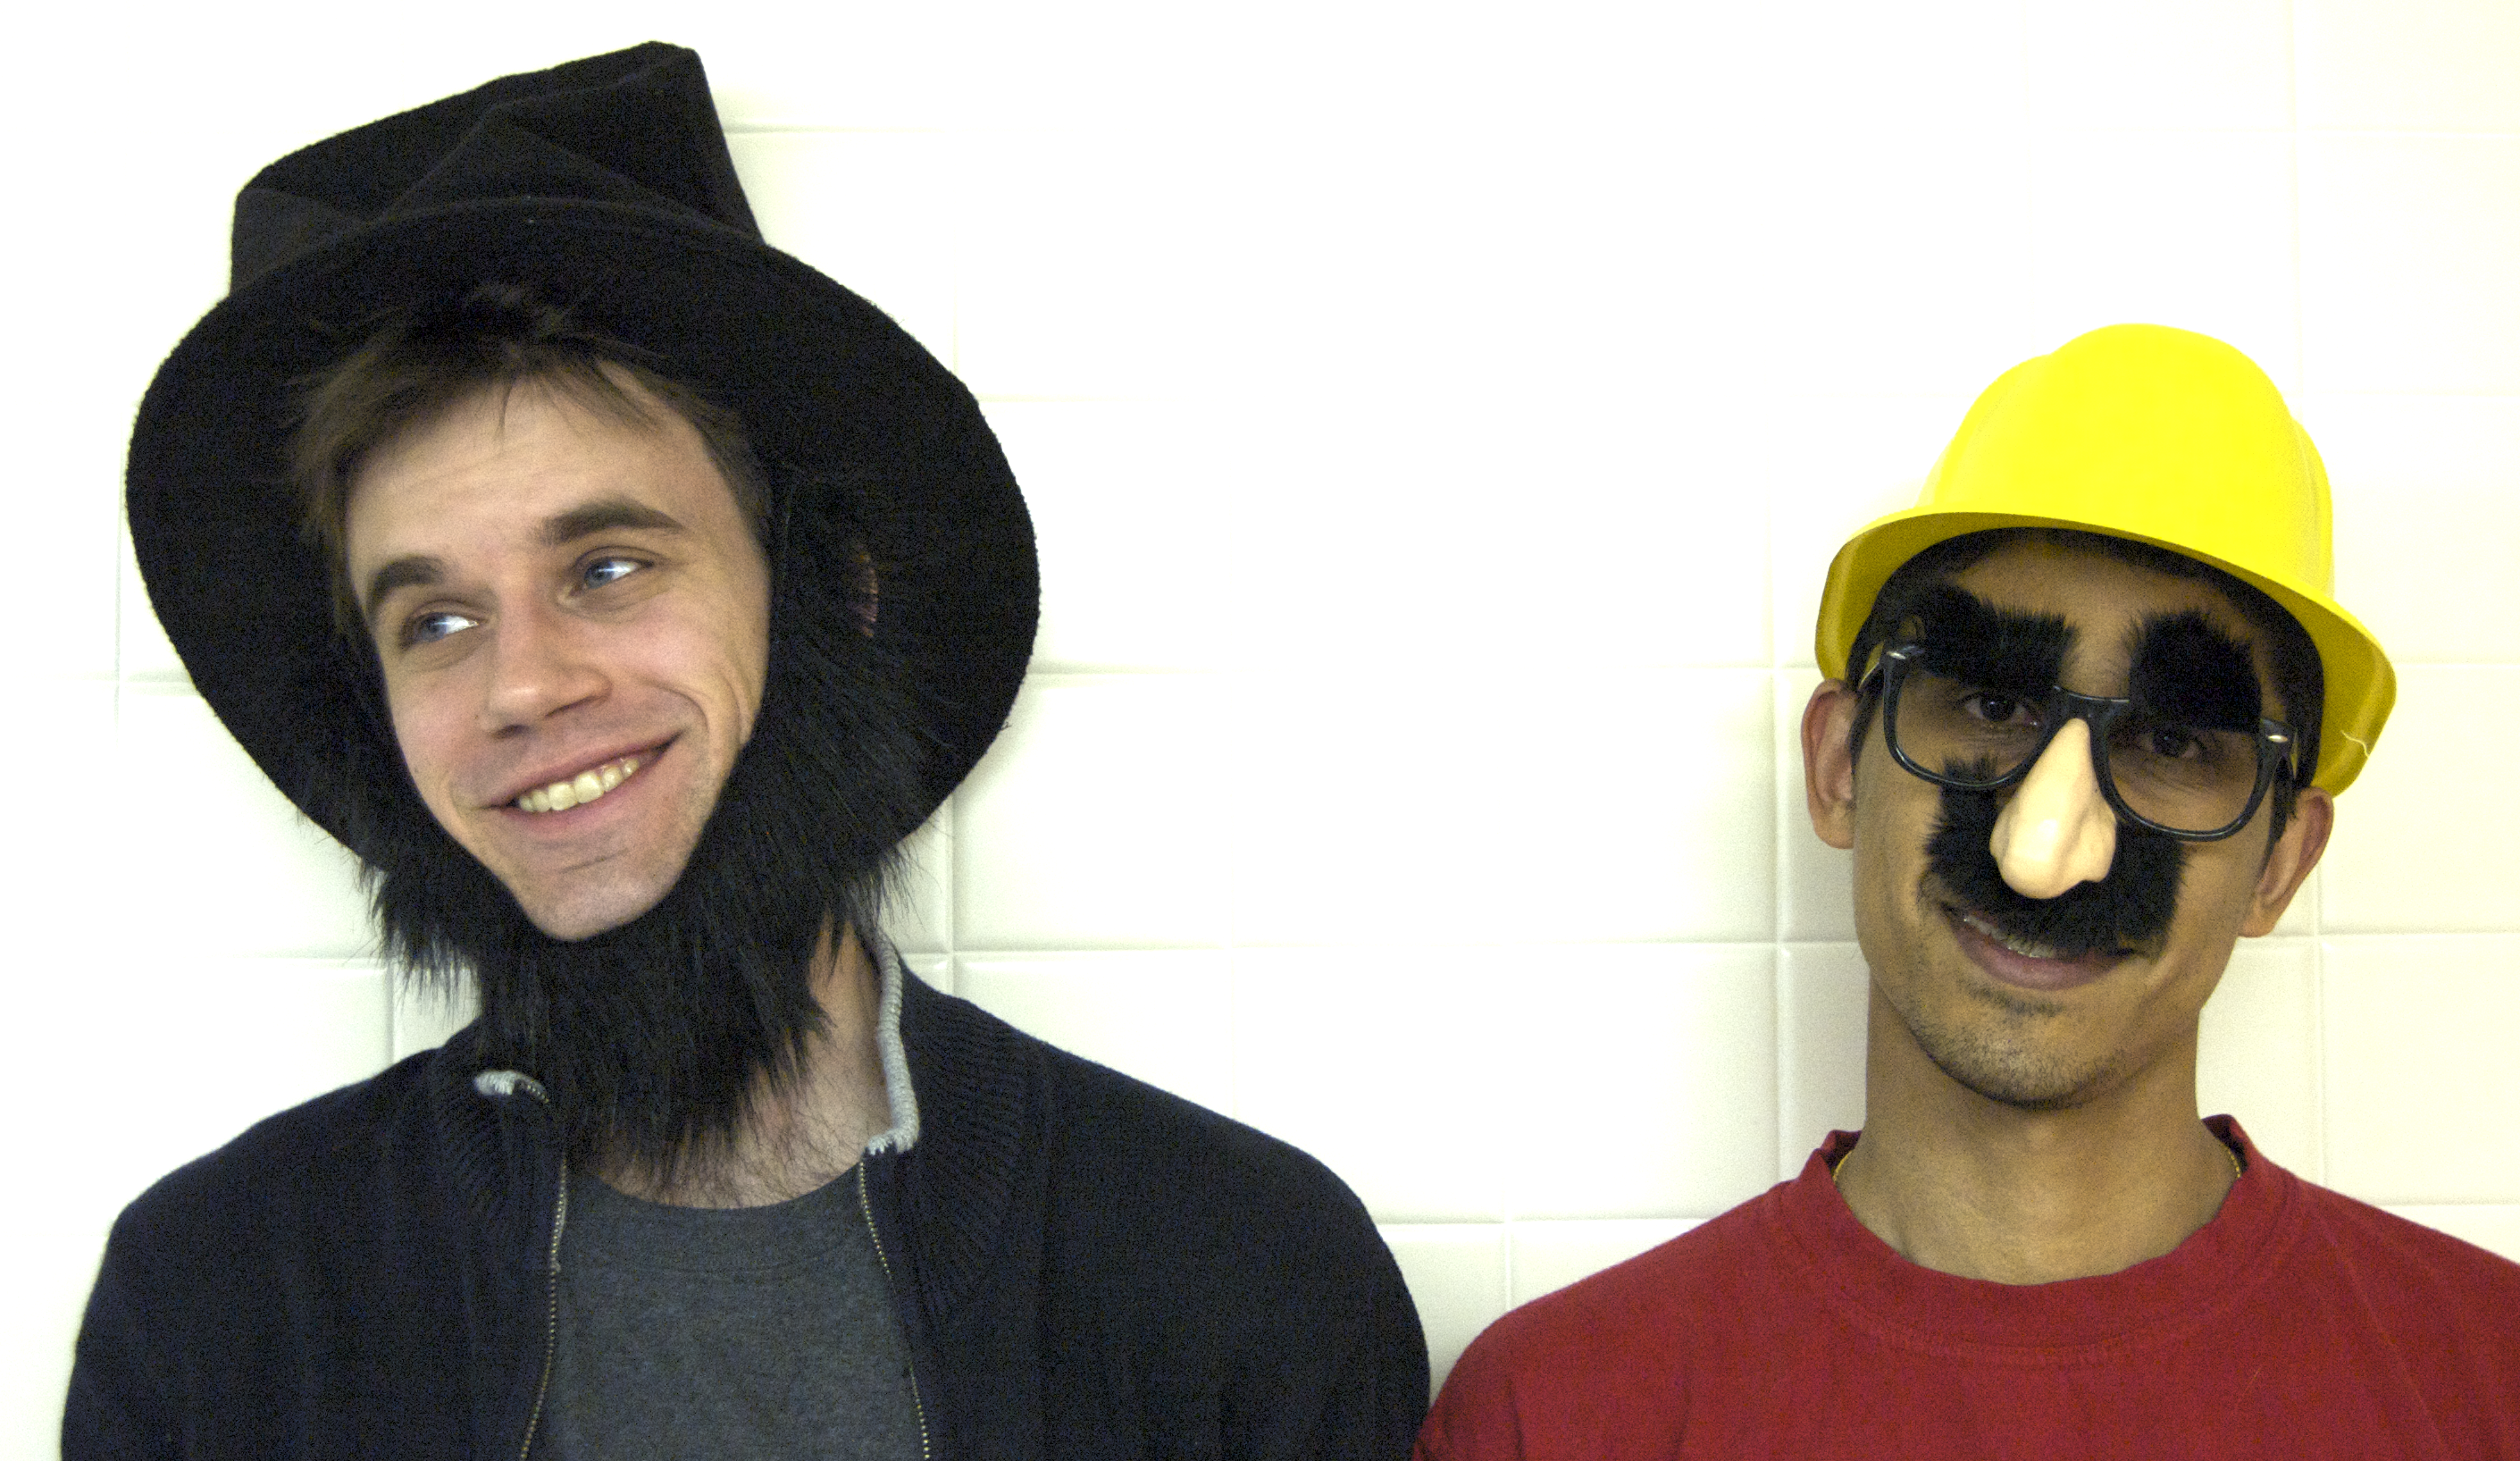
\includegraphics[width=.4\textwidth]{images/bathroom/tiltheads.png}}
\end{center}
}


